\section{Perceptrón}

El perceptrón fue la primera red neuronal artificial (o ANS, Artificial Neural Systems) descrita algoritmicamente. En las decadas de los 60's y 70's, los popularizo el psicólogo Franck Rosenblatt, en su libro llamado Principios de neurodinámica, donde presentó varios modelos de perceptrones.

El perceptrón es en sí, es la representación de un sola neurona, este se ocupa para la clasificación de patrones en un conjunto de datos multivariados, con ese se obtienen fronteras lineales en el plano, mediante un algoritmo de aprendizaje que veremos más adelante.

Recordando, una neurona es un celula elemental que a partir de un vector de entrada procedente del exterior o de otras neuronas (estimulo), proporciona una única respuesta (si activo el potencial de acción o no), ver figura \ref{fig:unaNeurona}. Los elementos que actuan en una neurona los podemos listar como:
\begin{itemize}
 \item \textbf{Entradas:} $x_{j}(t)$. Las variables de entrada y salida pueden ser binarias (digitales) o continuas (analógicas) dependiendo del modelo de aplicación.
 \item \textbf{Pesos sinápticos:} $w_{ij}$. Representan la intensidad de interacción entre cada neurona presináptica j y la neurona postsináptica i.
 \item \textbf{Regla de propagación:} $h_{i}(t) = \sigma(w_{ij}, x_{j}(t))$. Proporciona el valor del potencial postsináptico, de la neurona i en función de sus pesos y entradas. 
    \begin{itemize}
     \item $h_{i}(t) = \sum_{i=0}^{n} w_{ij} x_{i} $, Es una suma ponderada de las entradas con los pesos sinápticos.
      Así, si la entrada es positiva, dependiendo de los pesos podemos saber si fue una sinapsis excitadora (pesos positivos) o inhibidora (pesos negativos).
    \end{itemize}

 \item \textbf{Función de activación o de transferencia:} $a_{i}(t)$ Proporciona el estado de activación actual, de la neurona $i$ en función de su estado anterior, $a_{i}(t-1)$ y de su potencial postsináptico actual. 
    \begin{itemize}
     \item $a_{i}(t) = f_{i}(a_{i}(t-1),h_{i}(t))$, es la que usalmente se usa.
     \item $a_{i}(t) = f_{i}(h_{i}(t))$, en algunos modelos solo se concidera que el estado actual no dependende del tiempo anterior.

     \end{itemize}

 \item \textbf{Función de salida: } $F_{i}(a_{i}(t))$ Da la salida actual, $y_{i}(t)$, de la neurona i en función de su estado de activación actual. El estado de activación de la neurona se considera como la propia salida. 
    \begin{itemize}
     \item $y_{i}(t) = F_{i}(a_{i}(t))$
     \item $y_{i}(t) = F_{i}(f_{i}(a_{i}(t-1),\sigma(w_{ij},x_{j}(t))))$
    \end{itemize}

\end{itemize}


\begin{figure}[h]
 \centering
 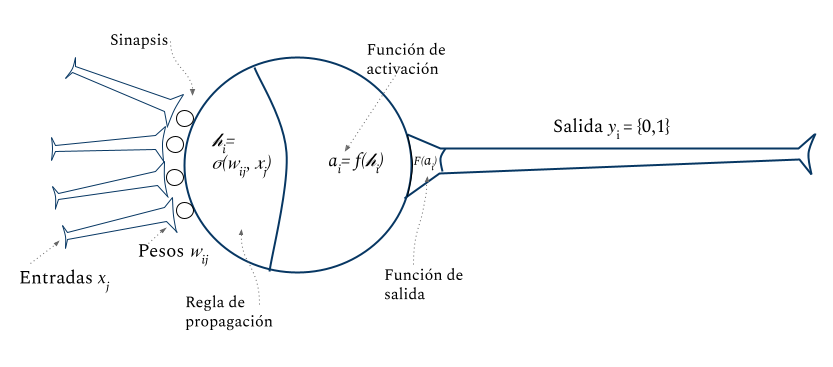
\includegraphics[scale=0.5]{../Figuras/Percp.png}
 \caption{Neurona vista como un modelo artificial (perceptrón).}
 \label{fig:unaNeurona}
\end{figure}


Un perceptrón toma un vector de entradas de numeros reales, calcula una combinación lineal de estas entradas, luego emite un 1 si el resultado es mayor que algún umbral y -1 de lo contrario. 
Es decir, dadas las entradas $x_{1}... x_{n}$, la salida $o(x_{1}. ..., x_{n},)$ calculada por el perceptrón es 1 si $w_{0} + w_{1}x_{1} + w_{2}x_{2} + ... + W_{n}x_{2} > 0 $ y -1 de lo contrario, donde cada $w$ es una constante $\Real $, peso, que determina la contribución de la entrada $x$ a la salida del perceptrón.  La constante $-w_{0}$ es un \emph{umbral} que la suma de las entradas con los pesos debe superar para que el perceptrón emita un 1. 
El hecho de que un perceptrón aprenda implica elegir valores para los pesos denotados también por $\theta$.  Ahora, el espacio $H$ de las hipótesis candidatas consideradas en el aprendizaje del perceptrón, es el conjunto de todos los posibles vectores de pesos.  \[H = {\vec{w} |  \vec{w} \in \Real^{n+1}\].

\begin{figure}[h]
 \centering
 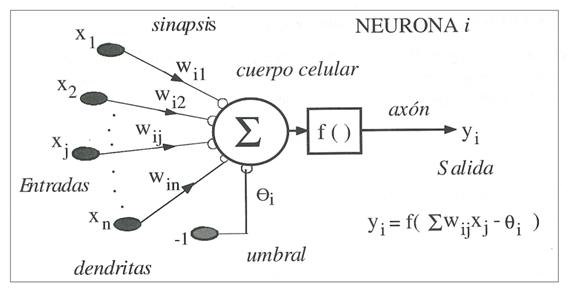
\includegraphics[scale=0.5]{../Figuras/neuronaPerceptron.jpg}
 \caption{Modelo estandar de un perceptrón. Me falta redibujarlo xD.}
 \label{fig:unaNeurona}
\end{figure}


